\chapter{Конструкторский раздел}
\label{cha:design}

Необходимо на данных алгоритмах разработать генератор и визуализатор облаков.

\section{Функциональная модель}

На рисунках \ref{img:idef0} и \ref{img:idef0_1} видно функциональные модели для генерации и визуализации облака.

\begin{figure}[H]
    \centering
    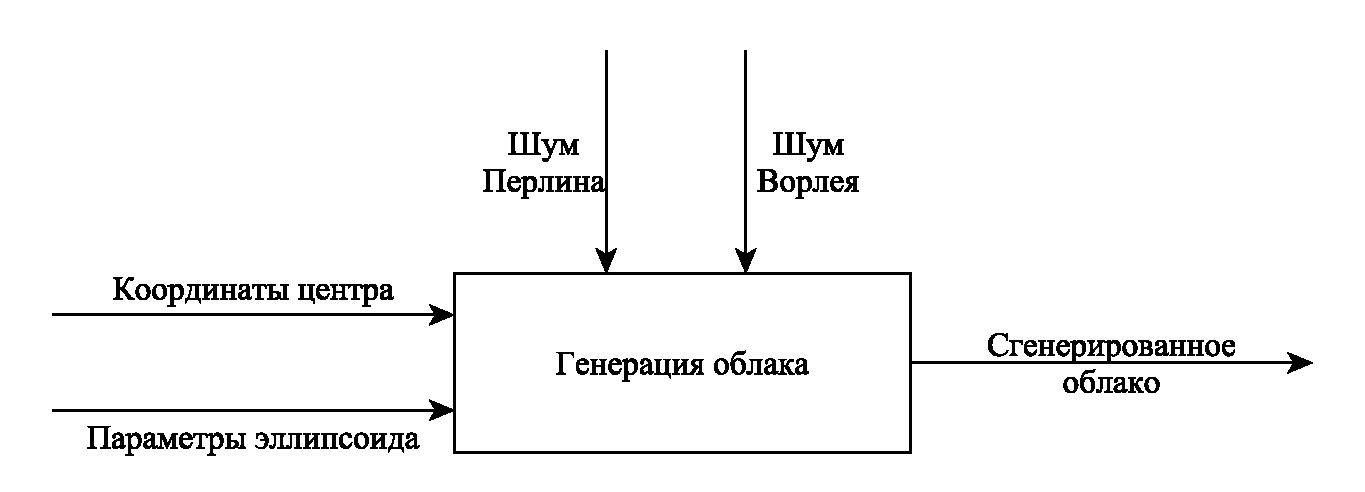
\includegraphics[scale=0.6]{img/idef0.pdf}
    \caption{Функциональная модель IDEF0 1 уровня для генерации облака}
    \label{img:idef0}
\end{figure}

\begin{figure}[H]
    \centering
    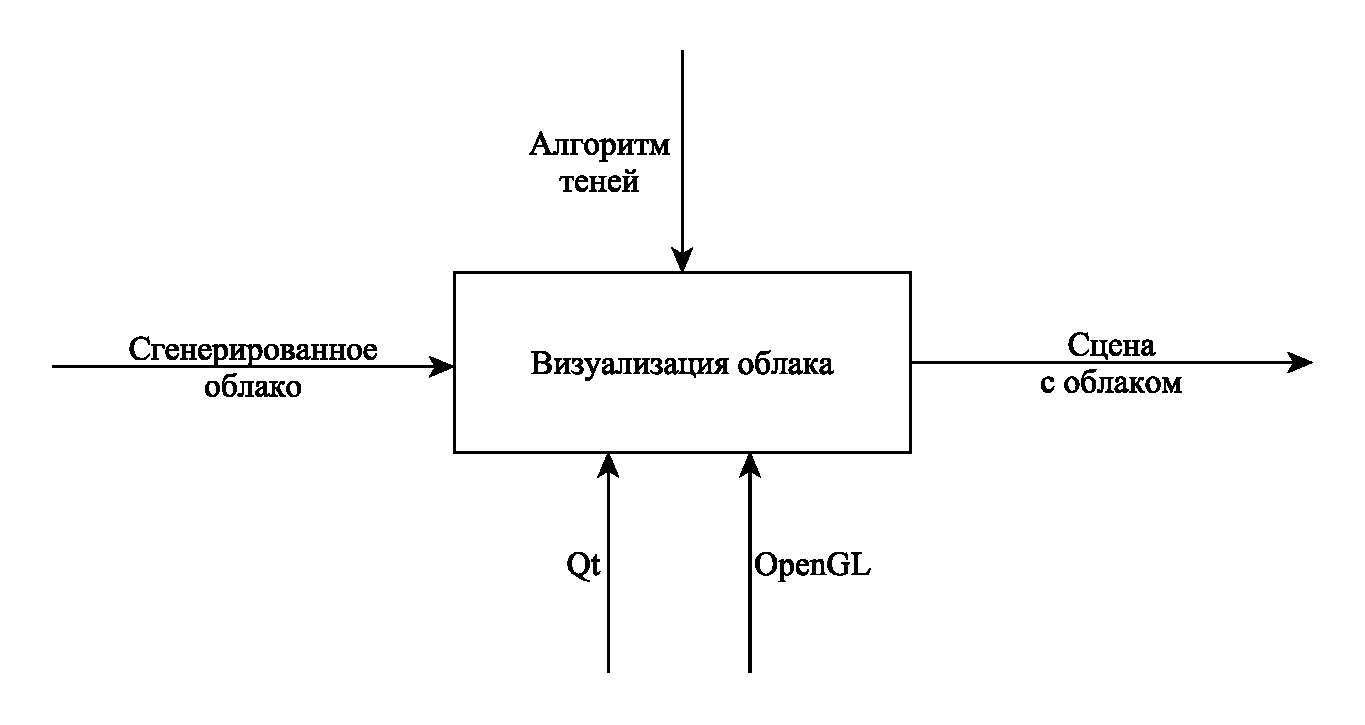
\includegraphics[scale=0.6]{img/idef0_1.pdf}
    \caption{Функциональная модель IDEF0 1 уровня для визуализации облака}
    \label{img:idef0_1}
\end{figure}

\section{Окружение}

Для создания окружающего пространства чаще всего используется куб больших размеров с наложенными текстурами.
Данный прием называется небесный куб. Куб создает впечатление об очень большом пространсве вокруг сцены и
существовании объектов, находящихся очень далеко \cite{SkyBox}.

\subsection{Форма облака}

Если из максимального значения интенсивности вычесть значение шума Уорли, можно получить результат как на рисунке \ref{img:worley2}

\begin{figure}[H]
    \centering
    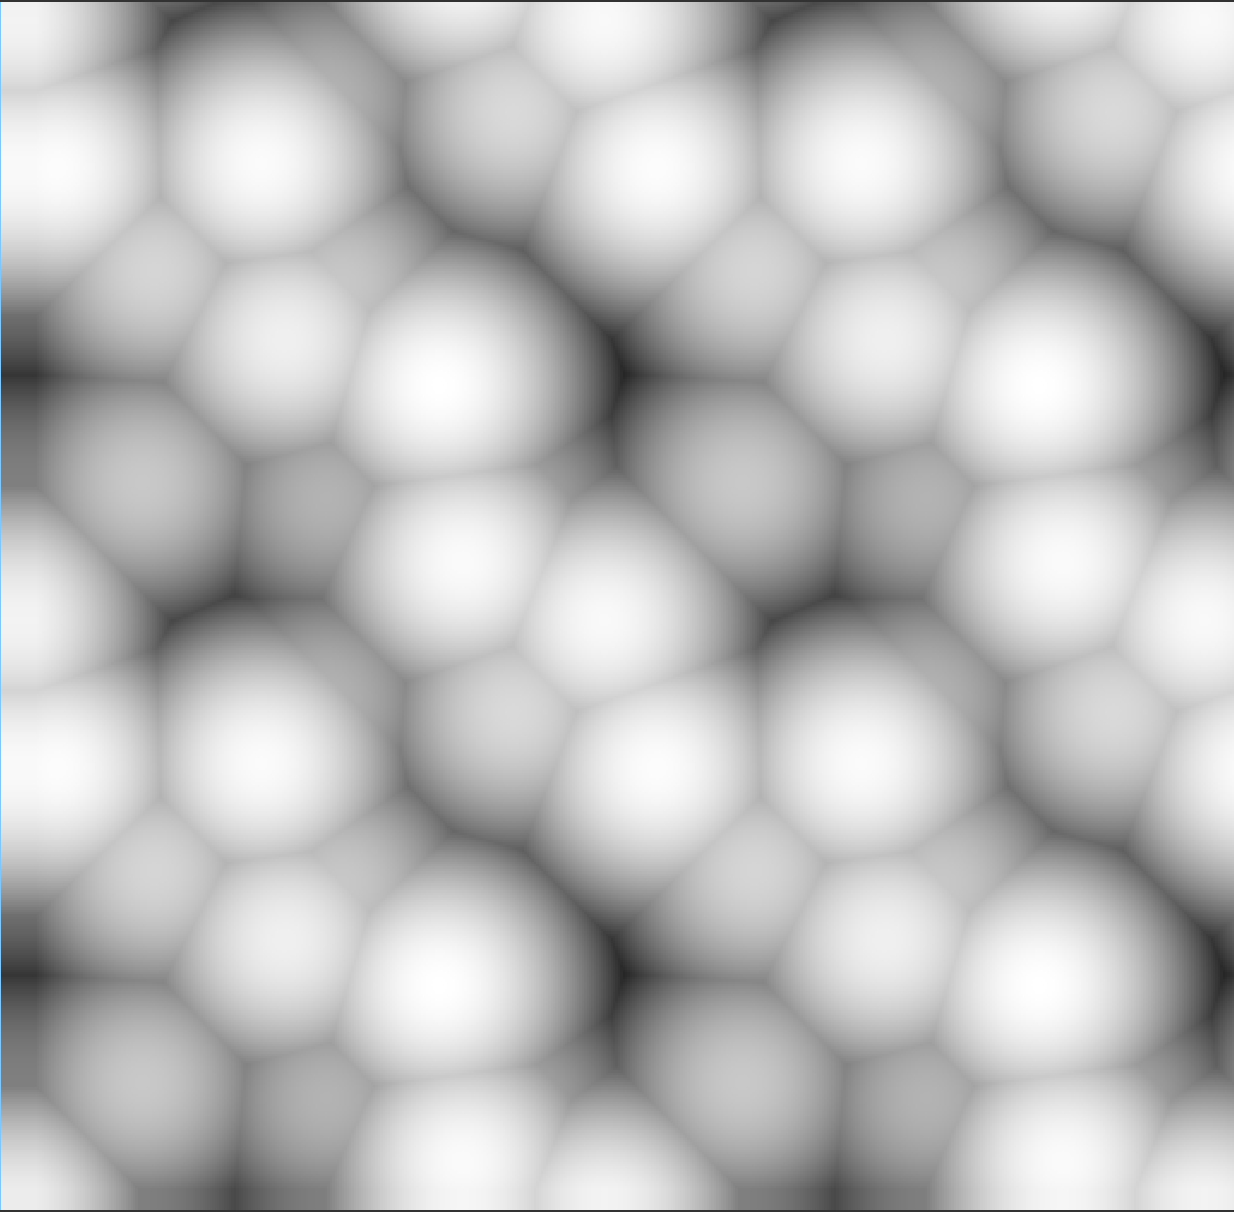
\includegraphics[scale=0.4]{img/worley2.png}
    \caption{Обратный шум Ворлея}
    \label{img:worley2}
\end{figure}

Если увеличить количество ячеек при генерации шума Уорли, можно получить результат как на рисунке \ref{img:worley3}.

\begin{figure}[H]
    \centering
    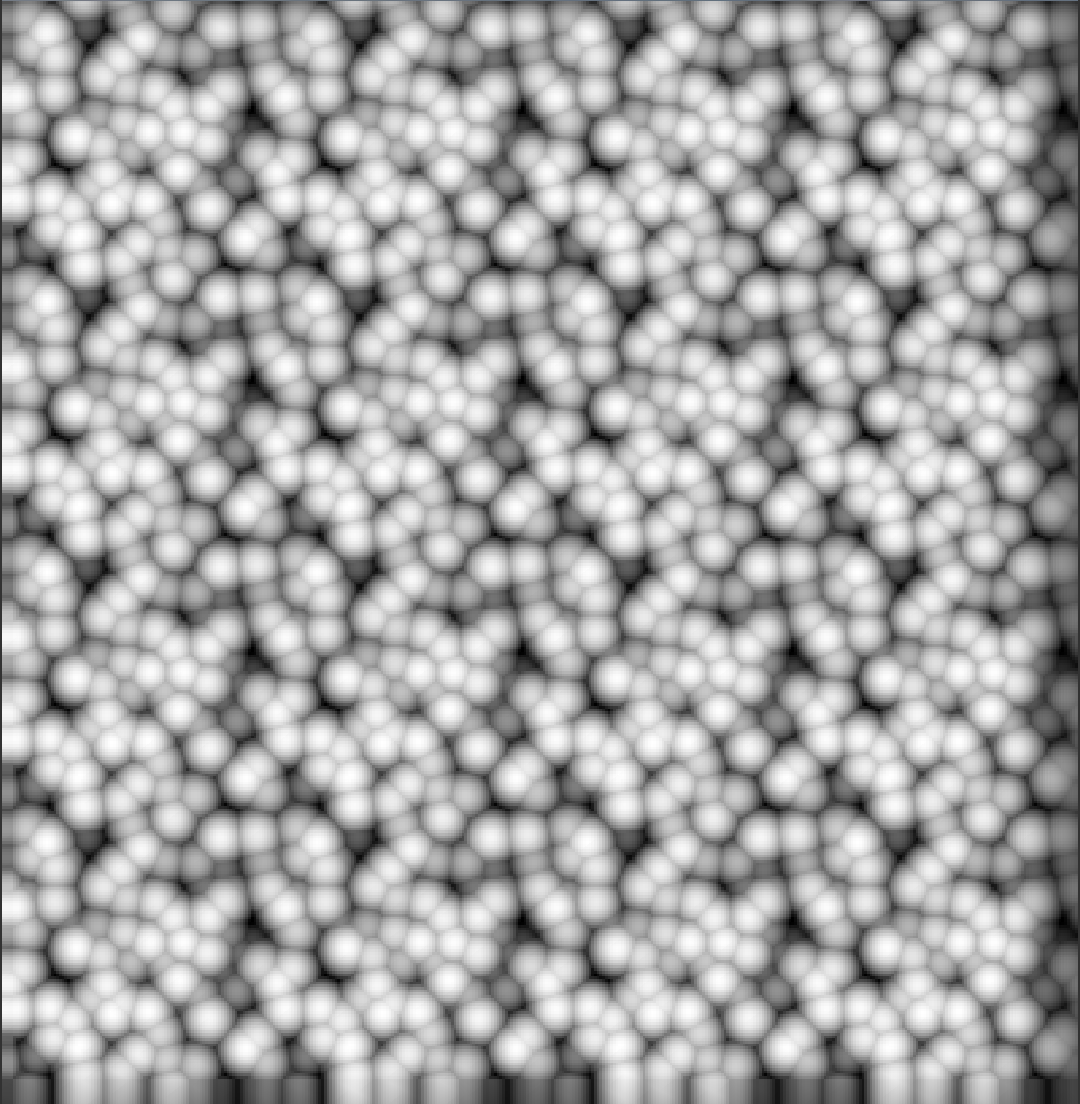
\includegraphics[scale=0.4]{img/worley3.png}
    \caption{Обратный шум Ворлея с большим количеством ячеек}
    \label{img:worley3}
\end{figure}

Для генерации облаков используется совмещение двух шумов. Шум Перлина придает
облаку случайную форму, а шум Ворлея - резкие очертания шарообразной формы.

Выведем формулу, в которой берется за основу шум Перлина, на который накладывается обратный шум Уорли первого варианта
(рисунок \ref{img:worley2}) и добавим к ним еще более мелкие шарики, взятые с шума Уорли, где больше ячеек (рисунок \ref{img:worley3}).
Экспериментальным методом была выведена данная формула \ref{eq:noise}.

\begin{equation}\label{eq:noise}
    \begin{matrix}
        F_{xyz} = P_{xyz}(20) + 0.1 + ((1 - W_{xyz}(4)) \cdot 1.5 - W_{xyz}(8) \cdot 0.7) \cdot 0.8 + P_{5x5y5z}(20), \\
        \text{где } P_{xyz}(n) - \text{ функция шума перлина после } n \text{ октав в точке } (x, y, z), \\
        W_{xyz}(n) - \text{ функция шума Уорли с плотностью ячеек } n \text{ в точке } (x, y, z) \\
    \end{matrix}
\end{equation}

Ее результат очень похож на облачную текстуру, которую можно увидеть на рисунке \ref{img:result_noise}.

\begin{figure}[H]
    \centering
    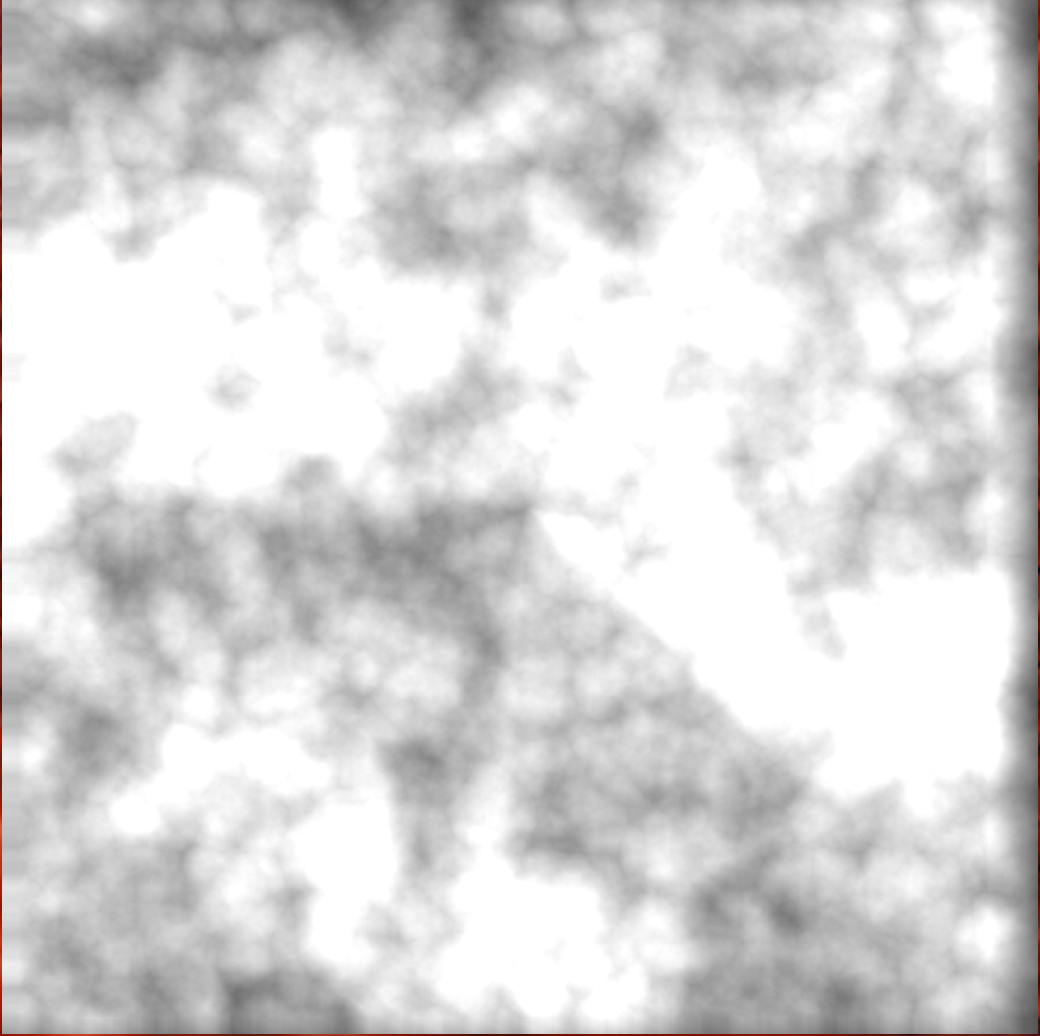
\includegraphics[scale=0.4]{img/result_noise.png}
    \caption{Результат объединения шумов}
    \label{img:result_noise}
\end{figure}

Для основы облака оспользуется параметрическое уранение эллипсоида, показанное на формуле \ref{eq:ellipsoid}
\cite{Ellipsoid}, в котором для каждой точки высчитывается новый радиус
по формуле \ref{eq:noise}. Поверхность эллипсоида получается очень похожей на облако.

\begin{equation}\label{eq:ellipsoid}
    \begin{cases}
        x = x_0 + a \cdot \sin(\Theta) \cdot \cos(\varphi) \\
        y = y_0 + b \cdot \sin(\Theta) \cdot \sin(\varphi) \\
        z = z_0 + c \cdot \cos(\Theta) \\
    \end{cases}
    , (-\frac{\pi}{2} \le \varphi \le \frac{\pi}{2}, 0 \le \Theta \le 2\pi)
\end{equation}

Параметры $a,b,c,x_0,y_0,z_0$ можно менять для получения разных размеров и местоположений облаков.

В зависимости от размеров облака, то есть от параметров $a, b, c$ выбирается шаг для углов $\Theta, \varphi$.
Поскольку размер каждой частицы составляет $0.1$, шаг был выбран $\frac{3}{\max(a,b,c)}$ для избежания
разрывов между частицами.

\section{Выводы}

Таким образом, был разработан алгоритм, основанный на шуме Перлина и шуме Уорли, которые влияют
на поверхность эллипсоида, получая объект, состоящий из частиц, который похож на облако.
